%\section{Description}
\label{merge}
Merging is a technique which takes two sorted lists, and combines them into a
single sorted list. Starting at the smallest key on both lists, it writes the
smaller key to a third list. It then compares the next smallest key on that list
with the next smallest on the other, and writes the smaller to the auxiliary
list. The merging continues until both lists are combined into a single sorted
list.

Mergesort works by treating an unsorted array of length $N$ as $N$ sorted arrays of
length one. It then merges the first two arrays into one array of length two, and
likewise for all other pairs. These arrays are then merged with their neighbours
into arrays of length four, then eight, and so on until the arrays are
completely sorted.

Mergesort is an out-of-place sort, and uses an auxiliary array of the same size
for the merging. Since a lot of steps are required, it is more efficient to
merge back and forth - first using the initial array as the source and the
auxiliary array as the target, then using the auxiliary array as the source and
the initial array as the target - rather than merging to the auxiliary array and
copying back before the next merge step.

The number of merges required is $log_2(N)$, and if this number is even then the
final merge puts the array in the correct place. Otherwise, the sorted array
will need to be copied back into the initial array.

\section{Base Mergesort}

\subsection{Algorithm N}
\label{Algorithm N}

For his base algorithm, LaMarca takes Knuth's algorithm N \cite{Knuth98}.
LaMarca describes this algorithm as functioning as described above; lists of
length one are merged into lists of length two, then four, eight, and so on.
However, algorithm N does not work in this fashion. Instead, it works as a
\n{natural} merge. Rather than each list having a fixed length at a certain
point, lists are merged according to the initial ordering. If it happens that
there exists an ascending list on one side, this is exploited by the algorithm.
While this results in good performance, the merge is not perfectly regular, and
it is difficult or impossible to perform several of the optimizations LaMarca
describes on it.

\subsection{Algorithm S}

Knuth's algorithm S is a \n{straight} merge, and works as described above. It has
15\% lower instruction count than Algorithm N\footnote{This is observed on
random data, which algorithm N is not designed for. On more regular data, or
semi-sorted data, this will probably not occur.}. Algorithm S, like algorithm N,
is a very difficult algorithm to modify. Knuth describes it in assembly, and
making the optimizations that LaMarca describes on it is more difficult than
rewriting the algorithm more simply. The rewritten algorithm, referred to from
here on as `base mergesort', is a simple higher level version of algorithm S,
and performs only slightly more slowly.

A disadvantage of this method is that if an array has slightly more than $2^x$
keys, an entire extra merge step would be required, which would considerably
slow the algorithm. This problem is shared by all other versions of mergesort
considered here, except algorithm N. However, since our tests use exact
powers of two as set sizes, this problem does not affect them. LaMarca,
however, used set sizes such as 4096000, which at times would suffer from this
type of problem.

\subsection{Base Mergesort}
\label{base mergesort}
Three optimizations are described by LaMarca for the base mergesort. Firstly, a
bitonic sort, as described in \cite{Sedgewick02}, removes instructions from the
inner loop. Every second array is created in reverse, so that the larger keys  
are next to each other in the middle. The smallest keys are at the outside,
meaning that the lists are iterated through from the outside in. As a result, it
is not possible to go outside the array, and it is not necessary to consider the
lengths of the arrays, apart from when setting the initial array indices. When
the first array is exhausted, it will point to the last key on the other array,
which will be larger than all other keys in that array. When both are
exhausted, the last key of both arrays will be equal. A check is put in, in this
case, and merging ends if both indices are the same. Figure \vref{Visual Sort}
shows a bitonic merge.

The overhead of preparing arrays to be merged is small. However, for small
lists, the overhead is large enough that it can be more efficient to sort using
a much simpler sort, such as insertion, selection or bubblesort. In Section
\ref{insertion is predictable}, it is shown that insertion sort is the fastest
elementary sort.  Sedgewick's quicksort uses this, and LaMarca recommends the
use of a simple inline pre-sort, which can be made from insertion sort. To make
lists of length four, the smallest of the four keys is found, and exchanged
with the first key, in order to act as a sentinel. The next three keys are
sorted with insertion sort. The next set of four keys is sorted in reverse
using the same method. It is possible to hard code this behaviour, in an attempt
to reduce the instruction count, but in fact the instruction count stays the
same, and the branch prediction suffers as a result.

Finally, the inner loop is \n{unrolled}\footnote{Unrolling a loop means
executing several steps of the loop between iterations and reducing the number
of iterations, which lowers the loop overhead and allows for better scheduling
of the instructions.}. There are actually two inner loops, and they are both
unrolled 8 times. The compiler is also set to unroll loops. However, the
observed difference between unrolling manually and compiler unrolling is up to
10\% of instruction count, so manual unrolling is used.

Overall, these three optimizations reduced the instruction count by 30\%.

\section{Double Tiled Mergesort}
LaMarca's first problem with mergesort is the placement of the arrays with
respect to each other. If the source and target arrays map to the same cache
block, the writing from one to the other will cause a conflict miss. The next
read will cause another conflict miss, and will continue in this manner. To
solve this problem, the two arrays are positioned so that they map to different
parts of the cache. To do this, an additional amount of memory the same size as
the cache is allocated, which can be expensive for small arrays. The address of
the auxiliary array is then offset such that $index(source) + index(auxiliary) =
C$.

%TODO what does this formula mean. look up LaMarcas paper

While this step makes sense, whether this is valuable is very much a platform
dependant issue. Since virtual addresses are used, it may be possible that the
addresses used by the cache are not aligned as expected. Even worse, an
operating system with an excellent memory management system may do a similar
step itself. The program's attempt to reduce cache misses could then increase
them. In the event that the \n{Memory Management Unit} in the processor uses
virtual addresses to index its cache, or has a direct mapping between virtual
and physical or bus addresses, then this problem is very unlikely. The
simulations presented in this project address the cache by virtual address, and
so this optimization is effective in this case.

The next problem considered is that of temporal locality. Once a key is loaded
into the array, it's only used once per merge step. If the data does not fit in
half the cache, then conflict misses will occur, and no temporal reuse will
occur at all. The solution is to apply a technique used in compilers called
\n{tiling}. Using this technique, an entire cache sized portion of the array will
be fully sorted before moving on to the next set. When all the sets have been
sorted in the manner, they are all merged together as usual.

It is also possible to avoiding the copy back to memory. In the event of an odd
number of merge steps, the auxiliary array will contain the sorted array, which
needs to be copied back. This can be avoided by pre-sorting to make lists sized
two or eight. A large increase of instruction count was realized by sorting to
lists of length two, so a length of eight was used. When an even number was
required, four was used.

The final improvement was to fully sort keys in the level 1 cache, before
continuing to level 2 cache as in the tiled mergesort. The expected improvement
is not as significant as in the case of the level 2 cache, since the penalty
for level 1 misses is not great. For this reason, this sort is called Double
Tiled Mergesort instead of Tiled Mergesort, however, it is referred to as both
in this report.

\section{Double Multi-mergesort}

Double Multi-mergesort has two phases. The first is the same as tiled mergesort, and
sorts the array into lists sized $C/2$. The second phase attempts to improve
temporal locality by merging these lists together in a single merge step. There
are $k$ lists and this is called a \n{k-way merge}. It is possible to do a
search across each of these keys, maintaining a list of indices to the smallest
unused key from each list. When there is a small number of lists, this isn't a
problem, however, when the number of lists increases significanty, the overhead
involved in this is substantial. It is necessary to check each of the lists, and
each key searched would cause a cache miss, since each array segment is aligned,
and map to the same cache block.

To avoid this, a priority queue is used. The smallest key from each list is
added to the queue, and then put into the final target array. This reduces the
problem of the search overhead, but does not reduce the problem of
\n{thrashing}\footnote{Thrashing occurs when two arrays are mapped to the same
cache block, and the constant access of one followed by the other causes every
access to be a miss.}.  To avoid this, an entire cache line is added at a time
to the priority queue. There will still be conflict misses, but there will be no
thrashing since the keys overwritten in the cache will not be needed again.

LaMarca used a 4-heap for his priority queue, and an 8-heap is used here, for
the same reasons as before. The heap is aligned, and a cache line
is put into the array each time. The smallest key is at the top of the heap,
and this is put into its final position in the array. The heap is then fixed.

LaMarca uses a special tag to mark the last key from each list inserted into
the array. No more details are provided on this, and a sorted list of length $k$
is used here, in its place.  If the key at the top of the heap is the same as
the smallest value in the list, another eight keys are added from the array
segment to which the number belonged. This continues until the array is full
sorted.

Using a sorted list instead of LaMarca's tagging leads to a variety of problems.
The reason the sorted list is used is that no details of the tagging is
provided. The sorted list is $k$ keys long, and only needs to be properly sorted
once. The next time it needs to be sorted is when a new line is added, but in
this case only one key is out of place, and can be put in place with a single
insertion sort run. This is linear at worst, and will have only 1 branch
misprediction.

When a list is fully consumed, the next keys inserted will be from the next
list. This could be fixed with a bounds check, however, since the lists are
bitonic, the next keys inserted are going to be the largest keys from the next
array. These will be added to the heap, and take their place at the bottom,
without harmful effect. A harmful effect is possible, though, when lots of keys 
with the same value are in the array. All these keys would be inserted at a
similar time, and when the first one is taken off the heap, a list would add
eight keys, even though it had just added eight. In this manner, the size of the
heap could be overrun. With random keys over a large range, as in our tests,
this is unlikely, and so this is not addressed.

The heap used for the k-way merge should result in a large increase in
instructions, and a significant reduction in level 2 cache misses. The addition
of the heap should not result in an increase in misses, since the heap is small
and will only conflict with the merge arrays for a very short time. The heap is
aligned as described in the previous chapter, and has excellent cache
properties. LaMarca estimates that there should be one miss per cache line
in the first phase, and the same in the second phase, although each miss will
occur in both the source and target arrays. This sums to four misses per cache
block, for a total of one miss for every two keys in the array.

\section{Results}
\subsection{Test Parameters}
The level 1 cache is 8k, so 2048 keys can be sorted in the level 1 cache.
262144 keys can be sorted in the level 2 cache. When arrays were pre-sorted,
they were pre-sorted to a size four, or eight if the number of passes was going
to be odd. These were reversed for the double multi-mergesort; since it does a
k-way merge into the source array, the sorted cache sized segments need to be in
the auxiliary array. An 8-heap was used for the multi-mergesorts.

\subsection{Expected Performance}

Algorithm N and algorithm S are included in the results for reference, but are
not discussed here.

The instruction count of mergesort is $O(NlogN)$, and does not vary
according to input. Multi-mergesort should have a significantly higher
instruction count once its threshold is hit.

The number of memory references is also $O(NlogN)$, and mergesort's cache
performance should be very regular, so long as the data set fits in the cache. Once
the data set exceeds the cache, the number of cache misses should leap. For
multi-mergesort, they should flatten out after this, perhaps with a slight
slope to take into account the conflict misses of the aligned array segments. The
fully associative caches should not have these misses, and the results should be
correspondingly lower. Due to their design, the double mergesorts should have
better performance than their counterparts.

The flow control of mergesort is very regular, but there is no way to predict
the comparisons. As a result the misprediction rate should be $O(NlogN)$ for
all but the multi-mergesorts, which should increase once the threshold is
passed.

\subsection{Simulation Results}
\label{Mergesort results}

\plot{merge}{}{}{Results shown are for a Direct Mapped cache.}{Results shown are
for a Direct Mapped cache.}{}{}

The number of instructions, shown in Figure \ref{merge instructions} is exactly
as predicted, with a 50\% spike at multi-mergesort. Level 2 misses, shown in
Figure \ref{merge level 2 misses} are also as expected, although the
multi-mergesort does not show the same improvement over tiled mergesort as in
LaMarca's results.

%TODO look over lamarcas results
The prediction results in Figure \ref{Branch Simulation results for mergesort}
are as expected. Very little variation exists between the types of mergesort. It
is noticeable, though, that the spike in branch misses due to the
multi-mergesorts is considerably lessened by the two level adaptive predictor.
The reason for this is not clear.

Despite the improvement in cache misses due to multi-mergesort, it still cannot
account for the increase in instruction count as a result, and it has a higher
cycle count on the Pentium 4 (see Figure \ref{merge cycles}) as a result. The
other sorts generally perform in $O(NlogN)$ time, with double tiled mergesort
being the fastest. Note that the alignment of the mergesort may not work as
desired due to the size of the cache. This was optimized for a 2MB cache, while
the Pentium 4 cache is only 256KB. This means that the two arrays are aligned to
the same cache block. However, since the cache is 8-way associative, this is not
serious, and should not result in a lot of thrashing.

The results presented here differ from LaMarca's results. In the case of
instruction count, both sets are nearly identical: the graphs are the same shape
and have similar ratios between the base and multi-mergesorts. The cache results
have a similar shape to LaMarca's, with a large increase in misses as soon as
the arrays no longer fit in the cache, and similar ratios between the base and
tiled versions.  But while LaMarca reports a very small increase in level 2
misses once multi-mergesort's data set is larger than the cache, the results
here show nearly the same jump as tiled mergesort. This results in half as many
misses as the base mergesort, while LaMarca shows nearly 10 times fewer misses
for his multi-mergesort.

As a result of this discrepancy, it is not a surprise that LaMarca's results
indicate that multi-mergesort is far faster than base-mergesort, but the same
results are not shown here. The increase in instruction count cripples
multi-mergesort, and tiled mergesort emerges the victor.

This is not to say that LaMarca's results disagree with those here. In fact, it
is noticeable that multi-mergesort's cache misses plateau at the edge of the
graph, while other mergesorts' misses continue to climb. This is in keeping with
both LaMarca's theory and results.

\section{Predictor results}

\afterpage{
\setcounter{subfigure}{0}
\thispagestyle{empty}
\clearpage
\enlargethispage{14em}
\vspace*{-5em}
\begin{figure}[H]
\begin{changemargin}
\subfigure[]{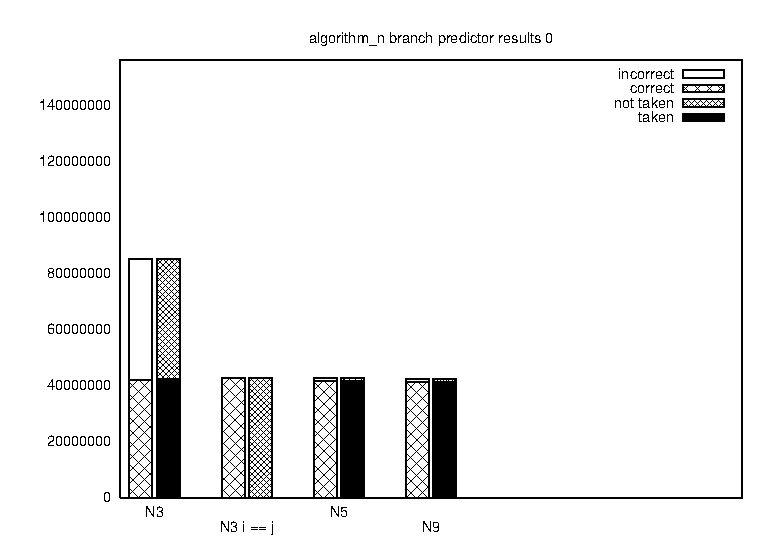
\includegraphics[scale=0.74]{../counters/algorithm_n-0.eps}}
\subfigure[]{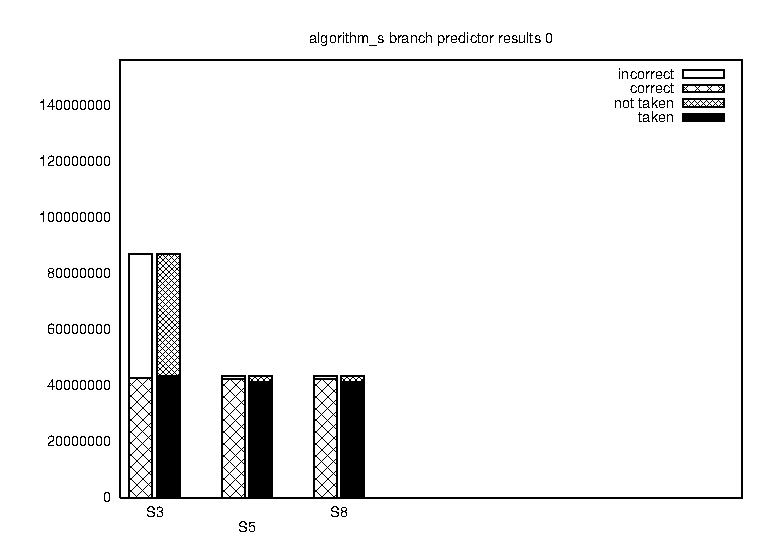
\includegraphics[scale=0.74]{../counters/algorithm_s-0.eps}}
\subfigure[]{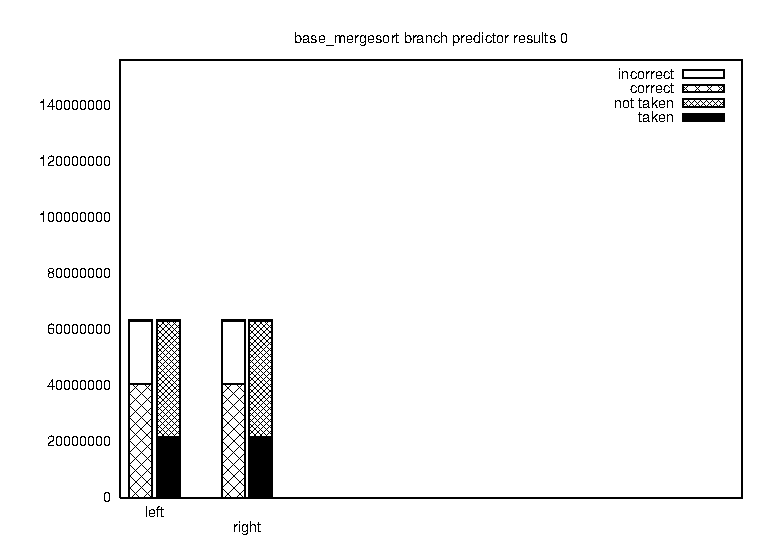
\includegraphics[scale=0.74]{../counters/base_mergesort-0.eps}}
\subfigure[]{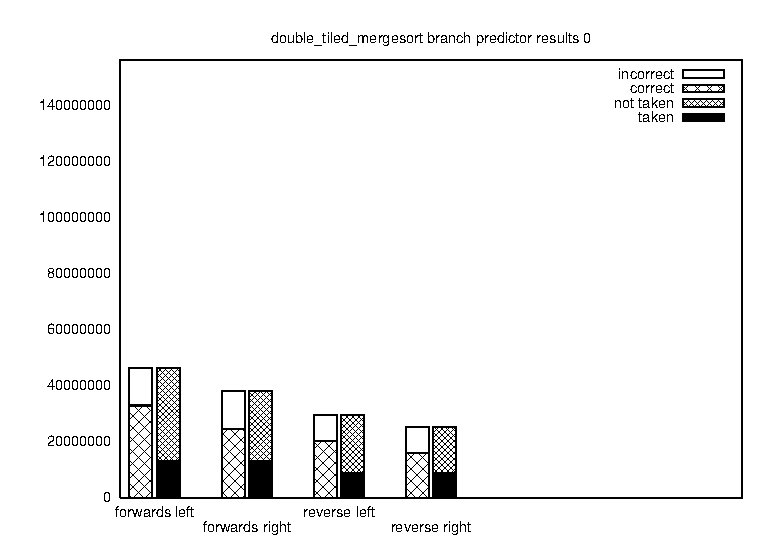
\includegraphics[scale=0.74]{../counters/double_tiled_mergesort-0.eps}}
\subfigure[]{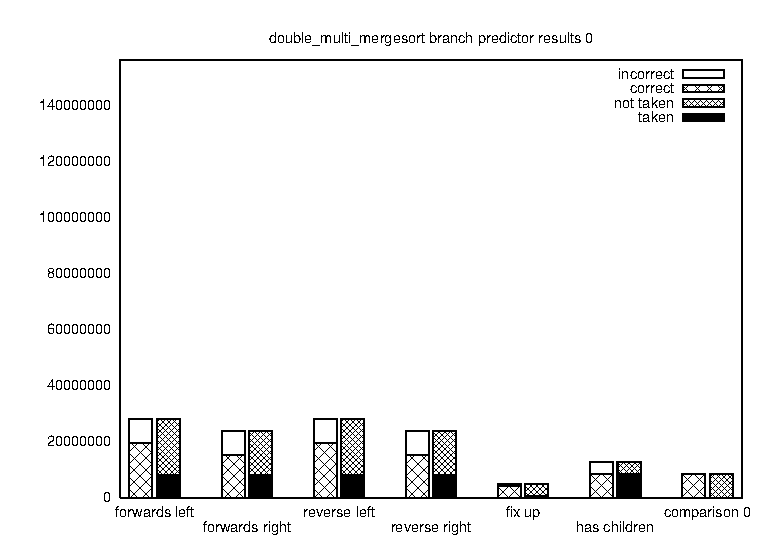
\includegraphics[scale=0.74]{../counters/double_multi_mergesort-0.eps}}
\subfigure[]{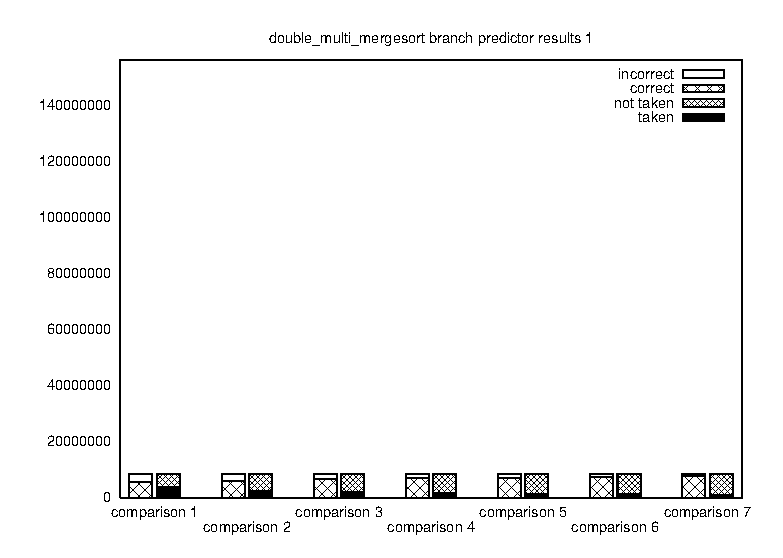
\includegraphics[scale=0.74]{../counters/double_multi_mergesort-1.eps}}
\end{changemargin}
\vspace*{6em}
\caption{Branch prediction performance for mergesorts. All graphs use the same scale.}
\label{Branch prediction performance for mergesorts}
\end{figure}
\newpage
}

%TODO This is a bit to rewrite

figure a shows Algorithm N, knuths natural merge. N3, N5 and N9 indicate parts of the flow chart. 'N3 i==j' is the second branch in N3.

The results show that the secondary loops are always taken. Taken here means broken out of, hence seldom used. The main action occurs in N3, the main comparator, which has a 50\% prediction ratio.

Algorithm S in graph B shows the same. I never really understood how it worked though.



Figure c shows base mergesort. This shows a lower number of branches and a higher percentage of correct predictions. The lower number of branches is probably due to the presort. there is a higher percentage of correct predictions, but the actual number of correct predictions in the same. This implies that doing the presort removes incorrect predictions (or, more to the point, moves incorrect predictions to another part of the algorithm). Note too, that both sides are used equally, which doesn't happen later. Two thirds of the branches are not-taken, which means loops execute twice before breaking. this is the same results that we found in quicksort later. I'm sure knuth explains this somewhere in the fine print.

Figure d shows double tiled mergesort. The total number fo branches is a 10\% increase over the base mergesort. Not sure why this is. 15\% increase in correct predictions so this incrase into predictable range, which should be avoidable (according to what we guess in quicksort).

Figure e and f show the double mulitmergesort results. This sorts fully within the cache only, reducing the number of branches relating to this. The reason that the previous balance was so muhc in favour of forwards was that the final sort at the end was forwards. Here though, the arrays are left bitonically, so there is an even distribution betwwen forwards and backwards. There si still the bias towards left rather than right. Left comes first in the code, but this doesnt quite explain why this happens. However, the number fo misses each way is identical.

The total branches is a decrease of about 20\% on base mergesort. The number of mispredictions decreases by less than 10\%. Howver, all these branches are made up by the increase in branches due to the heap. The number of extra brnahc misses due to this is 26\% of the branches misses in base mergesort. In total, the num ber fo branches isa equivalent however. So no loss by doing this (except lots of extra instructions, as seen before).

Note that here and in the heaps, comparison 0 does nothing. THe compiler ought to trim it out, except that now it actually does something (increases the branch counter).


finally, in base mergesort, there is an inline presort used. For efficiency, an insertion sort is used later. However, there are 6.8 misses per key in the inline presort, which is less than the insertion sort does. Its not as useful for presorting to 8, however. THese results hold forwards and in reverse.


%TODO up to here

\section{Future work}
Several avenues could be pursued in order to improve the algorithms presented
here. In multi-mergesort, LaMarca spoke of tagging keys as they went into the
cache. Here, a sorted list was used in its place. Implementing and investigating
tagging and comparing of the results of the two techniques would be interesting.

Algorithm N is a mergesort for more natural layouts of data, such as partially
sorted lists. It can sort these faster than a straight merge, but won't on
random data until it is nearly sorted. Some of the improvements described here
may be able to improve its performance, as they did for the straight merge.

To address one of the problems with multi-mergesort, that of the conflict misses
on the k-way merge, \cite{Xiao00} reveals a padded multi-mergesort with reduced 
conflict misses. It would be interesting to compare these results.

It may also be possible to simply reduce the number of conflict misses of the
k-way merge, simply by reducing the size of the initial sort by the size of
several cache lines. In this way, the smallest keys would map to different
cache blocks, without the need for padding.

%TODO
TODO what about level 1 cache misses if we realigned by 1024?
